Wind turbines and solar panels are carbon-free facilities and have become promising candidates for sustainable electricity generation. 
However, the uncertainty of wind and solar energy, which mainly comes from the difficulty of accurate long-term prediction, presents a significant challenge to traditional power scheduling system, such as infeasible or suboptimal solutions caused by day-ahead prediction errors~\cite{jabr2014robust}. The future power grids require a transformation in scheduling systems toward real-time decision-making to better utilize accurate ultra-short-term forecasts and tap the grids' flexibility. Such real-time requirement is not possible with the current computationally heavy scheduling algorithms.
In this research, we propose a reinforcement learning(RL) based real-time scheduling framework on the top of MuZero series' work.
Experimental results show that our approach significantly reduces renewable generation curtailment while ensuring the stable operation of a power system with high penetration of renewable energy. Moreover, our proposed approach is proved to save billions of dollars in costs for thermal generator flexibility retrofits and energy storage construction.

  
In traditional power systems, power generation schedules are calculated by the day-ahead scheduling(DAS) program, which is often done a day or several days in advance. It consists of two stages of work. First, based on day-ahead forecasts of load and renewable generation, the start/stop schedules of thermal generators are determined by solving a so-called day-ahead unit commitment(UC) problem. Second, according to the real-time load and renewable generation, the output power of generators at each time step is optimized economically to minimize the generation costs, while satisfying the operational security constraints of power grids, which is called the intraday economic dispatch(ED) problem.
Such a procedure is practical since the power output of traditional power plants, such as fossil fuel plants, are entirely under human control, and the load prediction is also well-developed. However, due to the hardness of accurately predicting the long-term power output of increasing renewable energy sources, it is difficult to guarantee that the results of day-ahead UC are feasible.
For example, once the renewable generation is overestimated, fewer thermal generators are set in service, which could lead to insufficient power ramping capacity, load shedding caused by mismatches between power generation and load consumption, or even system failures. 
On the other hand, underestimates of renewable energy may lead to excessive thermal units in operation, which results in renewable energy curtailments.



Under the above limitations of DAS, operators either choose to utilize renewable energy conservatively or execute flexibility retrofits to thermal generators and expand storage to increase the scheduling resources of power grids. 
Although the former requires real-time adjustments that can be done manually by human operators, the effectiveness and safety are highly dependent on their experience. The latter, while very effective in enhancing the grid's flexibility, requires a significant investment. 
Moreover, the retrofitted thermal units are likely to operate at non-economic operating conditions outside of their design specifications, instead increasing carbon emissions and costs per megawatts~\cite{chen2021flexible}. 
It is not efficient to implement future grid scheduling either by manual modifications or hardware upgrades.
Consequently, we want to investigate an innovative scheduling framework to deeply explore the flexibility of the existing grid.

One promising direction is incorporating precise ultra-short-term forecasts with the scheduling system to make real-time deisions.
Benefiting from the development of deep learning techniques, ultra-short-term forecasting of renewable energy generation has reached a dependable accuracy in recent years~\cite{wu2021ultra,tawn2022review}. 
However, the traditional DAS framework is difficult to schedule generation in such a short period of time.
Therefore, each control center requires a computationally fast algorithm that optimizes the power flow through real-time control of output power and starts/stops of generators, which is defined as the Real-Time Scheduling(RTS) problem. 
RTS is vital to utilizing the existing renewable energies and laying the foundation for broader applications in the future.  


To solve the RTS problem, we first reformulate it as a sequential Markov Decision Process (MDP), inspired by some work modeling scheduling as a finite-horizon optimal control problem~\cite{chandy2010simple}. On the basis of this concept, we build a RL environment based on a provincial power grid, along with actual load and power generation data. 
\shaohuai{This environment considers the optimization of AC power flow. 
}
The RL agent is allowed to obtain short-term predictions of load and renewable energy maximum power from the simulator to fit the ultra-short-term prediction's setting. The parameters of the transmission lines are also the same as the actual devices. The modifications are minimally added for data security reasons. This environment is named GridSim. 


On the algorithm side, 
instead of running an off-the-self reinforcement learning algorithm\shaohuai{Is this claim necessary? Maybe 'We refer to MuZero series' work and design....'}, we design a dedicated reinforcement learning algorithm for the Real-Time Scheduling problem, which we named GridZero. There are two major components in the GridZero algorithm. The first component is a fast neural network that can output near-optimal power grid scheduling operations. The second is a systematic search process that validates the proposed grid scheduling operations by simulating how the grid will change after the proposed operations. The search process could avoid the case when the current operation is valid but leads to future grid states that are hard to deal with. These two components are reminiscent of how an experienced power grid manager operates the grid: the operators intuitively know some good candidate controlling options according to their past experience, and then they validate the operation by further simulations. GridZero is inspired by the AlphaGo series' work, which excels at the game of Go~\cite{silver2016mastering,li2018alphago,silver2017mastering,schrittwieser2020mastering}. It seems that there is no relation between the game of Go and the power grid scheduling problem. However, we point out that both are highly complex sequential decision-making problems, and both significantly benefit from planning for the future. 

In summary, our method formulates the RTS problem as a Markov Decision Process, and we design a dedicated reinforcement learning algorithm. It avoids the load shedding of overestimating renewables and reduces the curtailment of renewable generation previously caused by underestimatings, both through the judicious use of ultra-short-term forecasts. Our method could better exploit the dispatching potential of the existing grid, and save huge amounts of costs in flexibility retrofits and storage construction. The proposed RL method also shifts the computational burdens from the iterative optimization process to an offline training process and achieves better solution quality simultaneously. Our algorithm could be one of the vital components of the future power grid that embraces renewable energies. 






\begin{figure}[h]
  \centering
  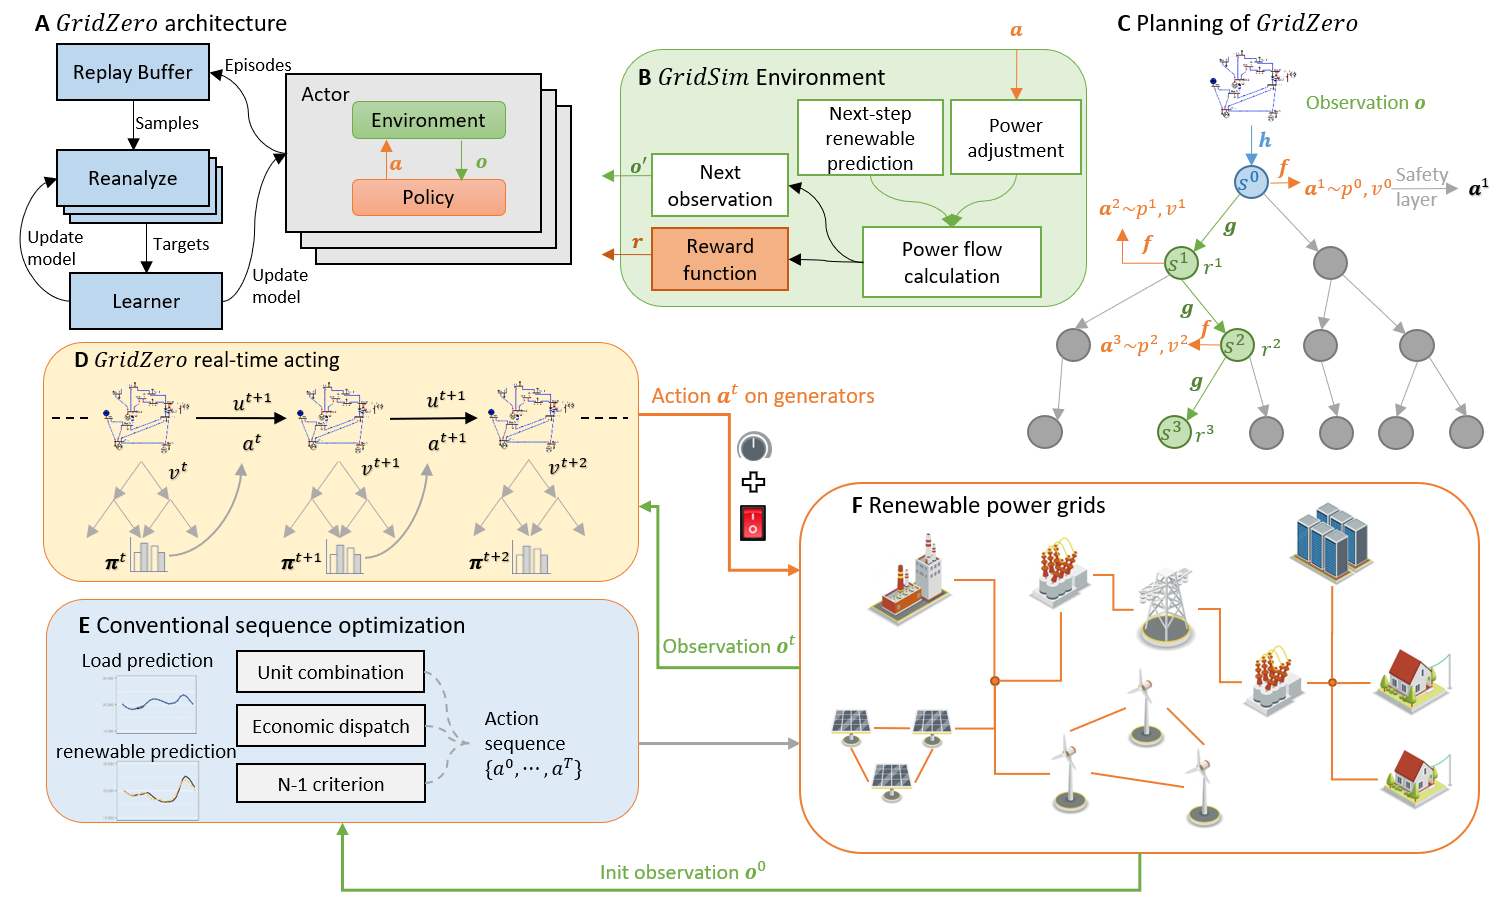
\includegraphics[width=0.85\linewidth]{fig/nature_fig1.png}
  \caption{\textbf{Representation of the components of GridZero design architecture.}
  \textbf{A}. Depiction of the training architecture. GridZero sends the scheduling action to GridSim based on the current grid observation. GridSim returns the next observation and the reward based on the power flow simulation result. These state transitions are sent to the replay buffer, which feeds data to reanalyze to make targets for the learner.
  \textbf{B}. GridSim interaction loop includes next-step renewable prediction, power flow calculation, and reward function.
  \textbf{C}. Our action selection is the result of a Monte-Carlo Tree Search process. The model consists of components for representation, dynamics, and prediction. Once a previous hidden state $s^{k-1}$ and an original action $a^k$ are given, the dynamics network $g$ can output an reward estimation $r^k$ and next hidden state $s^k$. The hybrid policy $p^k$ and value estimation $v^k$ are computed by the prediction network $f$ using the hidden state $s^k$. The candidate actions $\{a^k_i\}$ are sampled from the hybrid policy $p^k$. Especially, root action candidates must be processed by the safety layer. The hidden state $s^k$ is embedded by the representation network $h$ by using the observation of the whole power grid $o^k$.
  \textbf{D}. GridZero acts in a sequential Markov decision process that outputs an action and receives an observation interactively. 
  \textbf{E}. The conventional DAS precalculates a sequence of scheduling solutions based on the precise day-ahead prediction of load consumption. However, this framework is challenged by the inaccurate day-ahead prediction of renewable generation.
  \textbf{F}. A schematic of a power grid with renewable energy. Wind turbines, solar panels, and thermal generators work together to deliver power to the load. 
  } 
  \label{fig:nature_fig1}
\end{figure}



\subsection*{Real-time scheduling as an RL problem}
This section shows how to reformulate the RTS as an MDP and solve it. The proposed MDP incorporates the ultra-short-term predictions perfectly, as well as the operational constraints and objectives.
For better understanding, our real-time scheduling framework is illustrated in Fig.\ref{fig:nature_fig1}. There are two major phases in the approach. Our first step is to formulate the RTS problem as an MDP and create an RL environment GridSim. Second, we propose a planning capable agent GridZero that interacts with GridSim to find near-optimal policies 
through meticulous search processes.
\subsubsection*{MDP formulation and environment design}
In the first phase, 
the MDP is modeled as follows:
\begin{enumerate}[label=(\arabic*)]
    \item Observations encode the grid operational states, including generator output power, load consumption power, line transmission power, bus voltages, etc. Observations also include the next-step prediction of renewable maximum power and load consumption.
    \item Actions are designed as combinations of continuous adjustments of generator active power output and the discrete unit starts/stops, which aims to optimize the economic dispatch and unit commitment simultaneously. In addition, the renewable generator is modeled as controllable to increase the feasible solution space. Its legal power setpoint space is $[0, P_{\text{max}}^t]$ where $P_{\text{max}}^t$ is the maximum power at step $t$. \shaohuai{Renewable energy curtailment is the difference between the actual power and the maximum power.}
    \item State transitions represent the dynamic process to the next state, and they are \shaohuai{modeled in AC power flow models and} simulated through a professional power flow analysis program. 
    \item The reward is a scalar function that measures the grid's current state under the criteria of specific constraints and objectives. It also penalizes actions that lead to undesirable states.
\end{enumerate}

The proposed RL environment GridSim is based on the applied power flow analysis program of China Electric Power Research Institute. In order to depict the characteristics of future grids with high penetration of renewable energy, GridSim introduces a modified provincial power grid, SG-126, which has 126 buses, 91 loads, and 54 generators, 17 of them are renewable. The maximum generation of renewable energy accounts for more than 70\% of load consumption. Operational transections, including load, renewable generation data, and generator power set-points, are from actual measurements over a whole year, with data points spaced at 5-minute intervals for a total of 105,120 operational transections. Training and test datasets are separated and consist of measured transections of 2 consecutive years, which ensures that the agent is supposed to capture the essential dynamic characteristics of the grid operation instead of overfitting the training dataset. 


\subsubsection*{Algorithm design on the top of MuZero series}
In the second phase, we design an RL algorithm with meticulous planning processes that solves the RTS problem,
as shown in Fig.\ref{fig:nature_fig1}a,b. The proposed RL environment considers operational rules especially the thermal power ramping limitations and start/stop minimum interval constraints which are not considered in some related works~\cite{zhou2021deep,yan2020real}.

The RL algorithm learns from simulated interactions. However, purely random explorations could lead to severe consequences in a mission with such high security requirements. In the power system operation, the most important constraint is to keep power generation equal to the load consumption. More precisely, the time-varieties of renewable maximum power and load consumption make the boundaries of the action space also dynamically changes over time. To overcome the time-varying power balancing constraint, we design a safety layer and exploit the planning advantages. The safety layer adds linear modifications on the illegal actions of root nodes, and then maps them to the feasible solution space. It is necessary because violations of power balancing lead to immediate episode overs, thus no further explorations could help to learn the dynamic boundaries and policy improvements. This is common in many other similar tasks with high safety requirements. 

The search procedure to find a carefully selected action candidate is to generate a growing search tree, as shown in Fig.\ref{fig:nature_fig1}c. At each simulation, we dive to a leaf node along the most promising path, consisting of the child nodes with the highest Upper Confidence Bound (UCB) scores. Once reaching the leaf, we sample action candidates from the hybrid policy and generate new nodes to do further planning with the help of dynamics, reward, and value functions. More specifically, the observation at each root node is embedded as a vectorized hidden state by the representation function. Then a discounted future cumulative reward and a hybrid policy are correspondingly calculated by the value function and the policy function, using the vectorized hidden state as input. Once the hybrid policy is determined, the concrete action candidates, including generator power set points and on/off switchings, can be sampled from the hybrid policy. At each node, the agent could choose the most promising candidate with the highest UCB score. The reward and dynamic functions could estimate the immediate return and next hidden state if the action is selected.


